\chapter{Adversarial Detection}
\label{chpt:detection}

% \newrefsection

In this chapter, we focus on adversarial attacks against object detection systems. The task of object detection consists of object localization and object classification. The object detection model locates the position of each object, as well as classifies which category the object belongs to. Besides attacking the classification task, we need to deviate localization results as well. Thus, it's more challenging than adversarial attacks against image classification.

Another challenge is where and how we apply the adversarial perturbation. Unlike image classification which receives static images as input, object detection systems usually receive a real-time video stream from the camera. Though we may have various ways to generate the perturbation, if we cannot apply the perturbation in real-time, it won't affect real-world applications.

Starting with an introduction to existing object detection models and related white-box adversarial attacks, then we try to achieve an online attack that generates the perturbation in real-time. Thereafter, we explore the possibility of generating a single universal perturbation that could attack all the frames received from a camera. Lastly, we introduce the WHite-box Adversarial Toolbox (WHAT) that integrates our attacks into an open-source toolbox, and how we optimize our attacks so that the perturbation can be applied in real-time.

\section{Introduction}

Deep neural networks have been widely adopted in the task of object detection, and achieving SOTA performance. However, it's no more a secret that deep learning models are vulnerable to adversarial attacks. It has been nearly 8 years since the first adversarial attack against neural networks \citep{goodfellow2015explaining}. We can fool a deep learning model by adding small perturbations to the original input image. The perturbation is unperceivable by human eyes but can lead the detection model to inaccurate results.

Based on where we apply the attack, current adversarial attacks can be classified into two categories: digital perturbation and physical perturbation. For digital perturbation, we apply perturbation in the digital world. The perturbation does not exist in the actual world. It is applied to the digital image captured by the camera. For physical perturbation, we apply the perturbation in the physical world. For instance, we print out the adversarial perturbation on a poster \citep{lee2019physical} or T-shirt \citep{xu2020adversarial}.

\begin{figure}[H]
\centering
\includegraphics[scale=0.8]{figures/chapter_detection/digital.png}
\caption{Digital Perturbation: The perturbation is added directly to the input image of the model.}
\label{fig.adv_digital}
\end{figure}

\begin{figure}[H]
\centering
\includegraphics[scale=0.45]{figures/chapter_detection/physical.png}
\caption{Physical Perturbation: The perturbation is printed on objects in real world.}
\label{fig.adv_physical}
\end{figure}

However, there are several disadvantages to both attacks. Digital perturbation is applied directly to the input image of the detection model \citep{lu2017no}. The problem is that the input of the model is inside the operating system, which we do not have access to. It's not trivial to hack into the system of Google's Self-Driving Car and apply the perturbation. As a result, the biggest hurdle for digital perturbation is that we cannot add the perturbation into a real system. This renders digital perturbation useless in practice. Research interests are shifting from digital perturbation to physical perturbation. 

% No need to worry about adversarial attacks

Inherent disadvantages exist for physical attacks as well. For physical attacks, the perturbation is inflexible and it's perceivable by the human eyes. Once the adversarial poster is printed out, we cannot change it unless we reprint it. This could take a long time during the trial-and-error process. Due to the inflexibility of physical perturbation, it may only work if the adversarial poster is placed within a limited range and from a specific perspective. As illustrated in Figure \ref{fig.adv_physical}, if the camera captures the image from another perspective, the adversarial poster becomes a normal poster. Besides, physical perturbations are perceivable by humans. Both adversarial posters and adversarial T-shirts look quite unusual compared with normal ones. Wearing an adversarial T-shirt on the street immediately draws others' attention. 

In summary, digital perturbation is flexible and inconspicuous, but impractical. Physical perturbation is more practical but inflexible and conspicuous. In this research, we would like to investigate if it is possible to bring digital perturbations to the real world so that we achieve a flexible and inconspicuous attack in the real world.

\subsection{Object Detection Models}

Before introducing adversarial attacks, it's worthwhile to get familiar with target object detection models. Existing frameworks of object detection can be categorized into two types: region proposal-based methods and regression/classification-based methods \citep{Zhao2019}. We can either solve localization and classification problems separately or simultaneously. If we first generate a series of region proposals and then classify each proposal into different categories, this is a region proposal-based method (Two-stage). On the other hand, if we regard object detection as a classification or regression task that outputs locations and categories simultaneously, this is a regression/classification-based method (One-stage). The PASCAL VOC dataset and MS COCO dataset are used for a benchmark among different models.

\begin{figure}[H]
\centering
\includegraphics[scale=0.6]{figures/chapter_detection/detection_review.png}
\caption{Two types of frameworks: region-proposal based (two-stage) and regression / classification based (one-stage) \citep{Zhao2019}.}
\label{fig.detection_frame}
\end{figure}

OverFeat \citep{overfeat2014} is one of the first papers that use Convolution Neural Network on object detection. They use a multi-scale and sliding window approach to scan over the image and find locations of objects in regression layers. This is computationally expensive as most sub-sections of the input image do not contain any object. A more efficient approach is to first generate region proposals, regions that could contain objects, and then extract features from these proposals for regression. Selective search \citep{uijlings2013selective} is a common approach to generate region proposals, and it's employed in R-CNN \citep{girshick2014rich} as well. 

\begin{figure}[H]
\centering
\includegraphics[scale=0.45]{figures/chapter_detection/rcnn.png}
\caption{The architecture of RCNN \citep{girshick2014rich}.}
\label{fig.rcnn}
\end{figure}

RCNN generates around 2000 region proposals using selective search. It's more efficient than the sliding window method, but still computationally expensive. The same author of RCNN then proposed Fast-RCNN \citep{girshick2015fast} to improve the efficiency. RCNN feeds 2000 region proposals into CNN to compute features, while Fast-RCNN only feeds the original input image once to the CNN to generate feature maps, making it more efficient. To further improve its efficiency, region proposal computation becomes the bottleneck. Thus, Faster-RCNN \citep{ren2015faster} employs Region Proposal Network (RPN) that takes an image of arbitrary size to generate a set of rectangular object proposals.

\begin{figure}[H]
\centering
\includegraphics[scale=0.4]{figures/chapter_detection/fast-rcnn.png}
\caption{The architecture of Fast-RCNN \citep{girshick2015fast}.}
\label{fig.fastrcnn}
\end{figure}

% FPN is not an object detector by itself. It is a feature extractor that works with object detectors. FPN extracts feature maps and later feeds into a detector, says RPN, for object detection. 

In contrast, regression/classification-based methods generate detection results in a single run, making it even more efficient. Region proposal-based frameworks consist of region proposal generation, feature extraction with CNN, classification, and bounding box regression. Different components are usually trained separately. This becomes the bottleneck for real-time applications.  Experimental results demonstrate that two-stage models are more accurate, while one-stage models are more efficient. Here, we introduce the two most widely deployed one-stage models: YOLO \citep{redmon2016you} and SSD \citep{liu2016ssd}. 

YOLO divides the input image into SxS grids. Each grid cell is supposed to predict objects at the center of each grid cell. To handle different aspect ratios of objects, YOLO predefines several anchor boxes at 3 different scales. Each grid cell outputs the confidence value, bounding boxes, and probability vectors of different classes. For example, if an input image of size 416x416 is divided into grid cells of shape 13x13, we have 32x32 grid cells in total. Suppose we have 9 predefined anchors, 3 at each scale, the YOLO model produces 32x32x9 = 9216 outputs, each output includes the confidence value, the position and shape of the bounding box, and the probability vector for each class. If we have 80 classes, each output is a vector of size 80 + 4 +1 = 85. All the outputs are then handled by NMS boxes to eliminate duplicated boxes and boxes that have a low confidence value of containing objects.

\begin{figure}[H]
\centering
\includegraphics[scale=0.6]{figures/chapter_detection/yolo.png}
\caption{The architecture of YOLO \citep{redmon2016you}.}
\label{fig.yolo}
\end{figure}

SSD is another one-stage detection model that can outperform Faster-RCNN on both PASCAL VOC and MS COCO dataset with hard negative mining, data augmentation, and carefully chosen anchors, but much more efficient.

\begin{figure}[H]
\centering
\includegraphics[scale=0.6]{figures/chapter_detection/ssd.png}
\caption{The architecture of SSD \citep{liu2016ssd}.}
\label{fig.ssd}
\end{figure}

However, both one-stage and two-stage models are vulnerable to adversarial attacks. In this research, we test adversarial attacks against both types of models. In other words, we choose Faster-RCNN, Mask-RCNN \citep{he2017mask}, YOLO and SSD as our target models.


\subsection{White-box Adversarial Attacks}

Adversarial attacks against object detection are still in their inchoate stage. The first adversarial attack against neural networks was published in 2014 that targets image classification models. A lot of following works on adversarial attacks have emerged since then. Most of them still attack image classification models. We find the first adversarial attack against image segmentation in 2017 \citep{fischer2017adversarial}, and an evaluation of the transferability of adversarial attacks against segmentation and detection \citep{gurbaxani2018traits} in 2018. More adversarial attacks against object detection arises since 2019, and most of them target two-stage detection models. More specifically, the Region Proposal Network (RPN) in Faster RCNN.

The Dense Adversary Generation (DAG) \citep{xie2017adversarial} method intends to misclassify objects by adding small perturbations to the input image. It deviates predictions of $n$ target objects from ground-truth class label $l_n$ by reducing the error between $l_n$ and $l^{'}_{n}$, where $l^{'}_{n}$ denotes adversarial labels that can be randomly sampled from other incorrect labels. The DAG attack against segmentation models is relatively easy because the attack can be achieved by assigning each pixel to a different class. While for object detection models that output several thousands of bounding boxes, fooling one bounding box is not enough as the rest could still make correct predictions. This problem is solved by attacking the Region Proposal Network (RPN) in FasterRCNN, where they increase the threshold of NMS in RPN, such that they attack several thousands of bounding boxes simultaneously.

The Robust Adversarial Perturbation (RAP) \citep{li2018robust} attacks the RPN as well. It fools the RPN to predict most objects as background and produces wrong estimations on bounding boxes even if correct foreground objects are proposed. This is achieved by optimizing the following loss function:

\begin{equation} 
min_\mathcal{I} \quad L_{label}(\mathcal{I};\mathcal{F}_{\theta}) + L_{shape}(\mathcal{I};\mathcal{F}_{\theta}), \quad s.t. \ \ PSNR(\mathcal{I}) \geq \epsilon
\end{equation}

\begin{equation}
    L_{label}(\mathcal{I};\mathcal{F}_{\theta}) = \sum_{j=1}^{m} z_j log(s_j)
\end{equation}

\begin{equation}
    L_{shape}(\mathcal{I};\mathcal{F}_{\theta}) = \sum_{j=1}^{m} z_j((\Delta x_j - \tau_x)^2 + (\Delta y_j - \tau_y)^2 + (\Delta w_j - \tau_w)^2 + (\Delta h_j - \tau_h)^2)
\end{equation}

The Unified and Efficient Adversary (UEA) \citep{ijcai2019-134} methods extends DAG with a feature loss to train a generative adversarial network (GAN) to generate adversarial examples. 

The above methods generate one adversarial perturbation for each image, thus the perturbation is image-specific. It is also possible to generate a universal perturbation that is image-agnostic. The adversarial objectness gradient attack (TOG)\citep{chow2020adversarial} iterates over the training set to generate a single perturbation that can fool all the images in the training set. The Universal Dense Object Suppression (U-DOS) \citep{LI2021107584} uses a similar approach, but it focuses on fooling objects to be the background. It is also possible to only attack specific objects using TAR \citep{mohamad2021}.

Here's a summary of the aforementioned adversarial attacks against object detection models:

- TAR \citep{mohamad2021} - 2021

- U-DOS \citep{LI2021107584} - 2021

- TOG \citep{chow2020adversarial} - 2020

- UEA \citep{ijcai2019-134} - 2019

- RAP \citep{li2018robust} - 2018

- DAG \citep{xie2017adversarial} - 2017

Though these methods generate digital perturbations, similar approaches can be utilized to produce physical perturbations. If we print out digital perturbations on a poster, it won't be a valid physical perturbation. Valid physical perturbations can be generated by adding extra constraints to the loss function, such as the Sub-sampled Non-Printability Score (SNPS). The Non-Printability Score (NPS) is employed to measure the error between a printed pixel and its digital counterparts. Thus the adversarial effect of digital perturbations can be preserved after being printed out.

In summary, different adversarial attacks define distinct loss functions that determine the objective of their attack. The loss functions are minimized in similar ways, and if we add constraints on the Non-Printability Score (NPS), we can generate phjmysical perturbations.

% \clearpage

\section{Real-time White-box Attacks in ROS}
\label{sec:adv_detect}

Intelligent robots rely on object detection models to perceive the environment. Following advances in deep learning security it has been revealed that object detection models are vulnerable to adversarial attacks. However, prior research primarily focuses on attacking static images or offline videos. Therefore, it is still unclear if such attacks could jeopardize real-world robotic applications in dynamic environments. 
This paper bridges this gap by presenting the first real-time online attack against object detection models. We devise three attacks that fabricate bounding boxes for nonexistent objects at desired locations. The attacks achieve a success rate of about 90\% within about 20 iterations. The demo video is available at \href{https://youtu.be/zJZ1aNlXsMU}{https://youtu.be/zJZ1aNlXsMU}.

Our objective is to fool the YOLOv3 \citep{redmon2018yolov3}, and YOLOv4 \citep{bochkovskiy2020yolov4} object detection models to mistakenly detect objects at locations where there is no object. We generate adversarial overlays by combining the imperceptibility of adversarial filters with the localizability of adversarial patches.

\subsection{Preliminaries}
\label{section_preliminaries}

This section clarifies the differences between adversarial filters and adversarial patches. Following this, we describe how prior research applies these filters and patches in the digital and physical world. \emph{Our} research focuses on applying adversarial patches in the digital world.

\begin{figure}[b]
    \centering
    \begin{subfigure}[b]{0.42\textwidth}
        \includegraphics[width=1\linewidth]{figures/chapter_detection/digital_filter.jpg}
        \caption{Digital filters apply the perturbation to the entire input image in the digital world \citep{wang2021daedalus}.}
        \label{fig:digital_filter}
    \end{subfigure}
    \begin{subfigure}[b]{0.42\textwidth}
        \includegraphics[width=1\linewidth]{figures/chapter_detection/physical_filter.jpg}
        \caption{Physical filters apply the perturbation by attacking the camera using, e.g., a translucent film attached to the camera lens \citep{li2019adversarial}.}
        \label{fig:physical_filter}
    \end{subfigure}
    \caption{Adversarial filters perturb the entire image.}
    \label{fig:filter}
\end{figure}

\subsubsection{The Adversarial Filter}

An adversarial filter refers to a perturbation added to the entire image. Thus, the adversarial filter is of the same size as the input image and is unperceivable by human eyes. Based on where we apply the perturbation, adversarial filters can be categorized as digital or physical filters.

\textbf{Digital Filter} (Fig. \ref{fig:digital_filter})

The first adversarial attack against image classification models was a digital filter that added a small perturbation to the entire input image \citep{goodfellow2014explaining}. The perturbation can be generated using either gradient-based methods \citep{madryMSTV18} \citep{kurakin2018adversarial} \citep{wong2019wasserstein} \citep{croce2020reliable} or optimization-based methods \citep{papernot2016transferability} \citep{carlini2017towards} \citep{qin2019imperceptible}. Prior research uses the $l_1$, $l_2$, and $l_{\infty}$ norms to measure the human perceptual distance between the adversarial and the original input image \citep{miyato2015distributional} \citep{sabour2015adversarial} \citep{chen2018ead}. While the digital filter first proved the existence of adversarial examples, it is limited in practical scenarios since it is not always possible to assume access to the input image.

\textbf{Physical Filter} (Fig. \ref{fig:physical_filter})

Physical filters attach a translucent film to the camera lens to perturb the entire image \citep{li2019adversarial}. While physical filters do not require access to the input image, they do require physical access to the camera. One big challenge with physical filters is the difficulty of manufacturing a film that precisely replicates the adversarial perturbation. Thus, the practical applicability of adversarial filters in the physical world is still rather limited. In addition, to the best of our knowledge, physical filters has so far only been used to attack image classification models, not object detection models. 

% \pagebreak

\begin{figure}[b]
    \centering
    \begin{subfigure}[b]{0.48\textwidth}
        \includegraphics[width=1\linewidth]{figures/chapter_detection/digital_patch.jpg}
        \caption{Digital patches replace a part of the input image with the adversarial patch (left top corner) \citep{liu2018dpatch}.}
        \label{fig:digital_patch}
    \end{subfigure}
    \begin{subfigure}[b]{0.48\textwidth}
        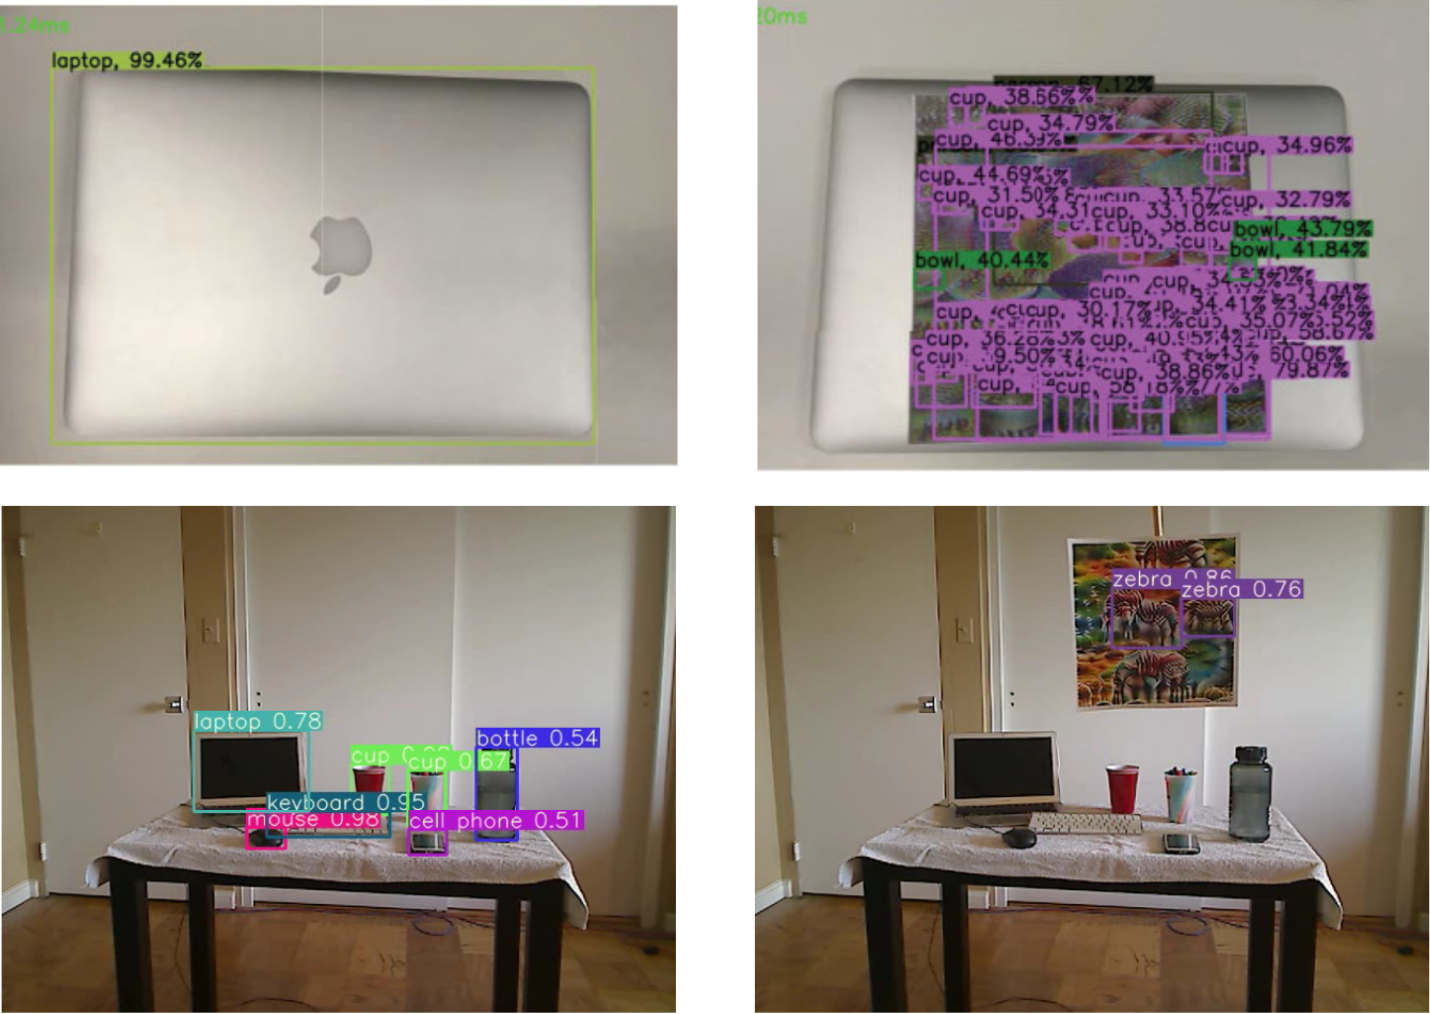
\includegraphics[width=1\linewidth]{figures/chapter_detection/physical_patch.jpg}
        \caption{Physical patches print the adversarial patch on a physical object, e.g., on a poster \citep{lee2019physical}.}
        \label{fig:physical_patch}
    \end{subfigure}
    \caption{Adversarial patches perturb part of the image.}
    \label{fig:patch}
\end{figure}

\subsubsection{The Adversarial Patch}

In some scenarios, it is possible to remove the constraint of the imperceptibility of the perturbation. This means that we can generate so-called patches that are clearly distinguishable to anyone viewing the image in question. 

Contrary to filters, these patches are limited in size and only perturb part of the image, allowing us to better control the location of generated objects when attacking an object detection model. Similar to filters, patches can be categorized as digital or physical patches.

\textbf{Digital Patch} (Fig. \ref{fig:digital_patch}) In 2018, Liu etc al. designed the DPatch \citep{liu2018dpatch} to attack the Faster R-CNN object detection model \citep{ren2015faster}. The DPatch is location-independent, which means that it can be placed anywhere in the input image. Another notable digital patch is the TOG attack, presented in 2020 by Chow et al \citep{chow2020adversarial}. They generated a 40x40 adversarial patch to fool object detection models into misclassifying objects to which the patch was attached.

\textbf{Physical Patch} (Fig. \ref{fig:physical_patch}) In 2017, Google presented landmark research for generating a physical patch to attack an image classification model \citep{brown2017patch}. As a result, research interest gradually shifted to from digital to physical patches. Later, Lee et al. \citep{lee2019physical} and Wang et al. \citep{wang2021daedalus} extended the physical patch attack from image classification to object detection. One shortcoming of physical patches is their inflexibility. Once the adversarial patch has been printed out, the only way to change it is through reprinting. To improve their flexibility, Hoory et al. dynamically displayed adversarial patches on a flat screen attached to a car \citep{hoory2020dynamic}.

% \subsection{Summary}

% Initially, research on adversarial attacks was focused on the design of digital perturbations. Later, adversarial attacks were extended the digital attacks to the physical world. In the next section, we describe a process for generating unperceivable digital patches at desired locations in real time.

% \clearpage

\subsection{Problem Formulation} 

The YOLO object detection model splits the input image into $S$x$S$ grids and makes predictions for each grid. For example, the input shape of YOLO is 416x416x3 (height, width, and channel). If $S=13$, we divide each channel into 13x13 grids, and each grid is 32x32 pixels. To detect objects of different sizes, YOLO makes predictions at three different scales (see Fig. \ref{fig.grid}). The first, second, and third output layer contains 13x13, 26x26, and 52x52 grids, respectively. The first output layer detects larger objects, and the third output layer detects smaller objects. In addition, YOLO pre-defines three anchor boxes ($B=3$) at each scale to detect objects of different aspect ratios. Thus, we have 9 pre-defined anchor boxes for 3 scales. Lastly, each output contains the shape and location of the bounding box, the confidence value, and the probability vector for each class (see Fig. \ref{fig.grid}). For example, if the model is pretrained on the MS COCO dataset \citep{mscoco2014} \citep{moore2020fiftyone} that contains 80 classes ($K=80$), each output contains 85 values consisting of four dimensions ($b_x, b_y, b_w, b_h$), one confidence value ($c$), and 80 probabilities $(p_1, p_2, ..., p_{80})$ for each class.

Putting things together: Given an input image $x$, the object detection model outputs $S$x$S$ candidate bounding boxes $o \in \mathcal{O}$ at three different scales ($S \in \{13,26,52\}$, $B=3$, and $|\mathcal{O}| = \sum_{1 \leq i \leq 3} S_i \times S_i \times B$, where $S_i$ represents the grid size of the $i_{th}$ output layer). Further, each candidate box is
\begin{equation}
 o^i = [b_x^i, b_y^i, b_w^i, b_h^i, c^i, p_1^i, p_2^i, ..., p_K^i],\ 1 \leq i \leq |\mathcal{O}|
\end{equation}
for $K$ classes. For example, the shape of the first output layer is $(S_1,\ S_1,\ B,\ K + 5) = (13,\ 13,\ 3,\ 85)$. The image is divided into 13x13 grids, and the model makes predictions for 3 anchor boxes. Each prediction contains 85 values (85 = 4 + 1 + 80). The adversarial attack aims to generate an adversarial perturbation $\delta \in [-1, 1]^{whc}$ such that the adversarial output $\mathcal{O}(x^{'})$ is different from the original output $\mathcal{O}(x)$.

\begin{figure}[b]
    \centering
    \includegraphics[width=0.5\textwidth]{figures/chapter_detection/grid.jpg}
    \caption{The YOLO object detection model makes predictions at three scales.}
    \label{fig.grid}
\end{figure}

% \pagebreak

\subsubsection{The Adversarial Overlay}

As described in Section \ref{section_preliminaries}, adversarial filters are imperceptible to human eyes but do not allow us to control exactly where in an image that we fabricate objects. Adversarial patches, 
on the other hand, are pinpointable but conspicuous. We propose a new method, the adversarial overlay, that applies an imperceptible perturbation to part of an image. Thereby, the adversarial overlay combines the strengths of adversarial filters and patches. The perturbations applied in filters, patches, and overlays can be contrasted as 
\begin{subequations}
\label{eq_perturbations}
\begin{align}
    x^{'}_{filter} &= x + \delta, \\
    x^{'}_{patch} &= (\mathbb{1}-m) \odot x + m \odot \delta, \\
    x^{'}_{overlay} &= x + m \odot \delta.
\end{align}
\end{subequations}
Here, the perturbation $\delta$ is applied via a binary mask $m \in \{0, 1\}^{wh}$, and $\odot$ is the Hadamard operator performing element-wise multiplication. As seen in equation \eqref{eq_perturbations}, the adversarial filter $x^{'}_{filter}$ applies the perturbation to the entire image without the mask $m$, the adversarial patch $x^{'}_{patch}$ uses the mask to replace part of the image, and the adversarial overlay $x^{'}_{overlay}$ applies the mask to the perturbation and adds it as an overlay to the image.

Now, note that the confidence value and the probability vector collectively determine whether or not a bounding box is drawn on the output image. Thus, by maximizing the product of confidence and probability vector, we can fabricate objects at desired locations. This leads us to propose three adversarial loss functions $L_{adv}$ for generating perturbations in real time: one loss function for one-targeted attacks
\setcounter{equation}{2}
\begin{equation}
\max_{1 \leq i \leq |\mathcal{O}|}\ [\sigma(c^i) * \sigma(p^i_t)] \label{eq:one-targeted},
\end{equation}
one loss function for multi-targeted attacks 
\begin{equation}
\sum^{|\mathcal{O}|}_{i = 1}\ [\sigma(c^i) * \sigma(p^i_t)] \label{eq:multi-targeted},    
\end{equation}
and one loss function for multi-untargeted attack
\begin{equation}
\sum^{|\mathcal{O}|}_{i = 1} \sum_{j=1}^{K}\ [\sigma(c^i) *\sigma(p^i_j)] \label{eq:multi-untargeted}.    
\end{equation}
Here, the function $\sigma (x)$ represents the sigmoid function.

% \begin{align*}
% One\ Targeted:\ \mathcal{L}_{adv}^{1}(\mathbfcal{O}) &= \sum^S \max_{1 \leq i \leq |\mathcal{O}|}\ [\sigma(c^i) * \sigma(p^i_t)] \\ 
% Multi\ Targeted:\ \mathcal{L}_{adv}^{2}(\mathbfcal{O}) &= \sum^S \sum^{|\mathcal{O}|}_{i = 1}\ [\sigma(c^i) * \sigma(p^i_t)] \\
% Multi\ Untargeted:\ \mathcal{L}_{adv}^{3}(\mathbfcal{O}) &= \sum^S \sum^{|\mathcal{O}|}_{i = 1} \sum_{j=1}^{K}\ [\sigma(c^i) *\sigma(p^i_j)]
% \end{align*}

%\begin{numcases}{\mathcal{L}_{adv}(\mathbfcal{O})=}
%\sum^B\max_{1 \leq i \leq |\mathcal{O}|}\ [\sigma(c^i) * \sigma(p^i_t)] & \label{eq:one-targeted}\\
%\sum^B \sum^{|\mathcal{O}|}_{i = 1}\ [\sigma(c^i) * \sigma(p^i_t)] & \label{eq:multi-targeted}\\
%\sum^B \sum^{|\mathcal{O}|}_{i = 1} \sum_{j=1}^{K}\ [\sigma(c^i) *\sigma(p^i_j)] \label{eq:multi-untargeted}& 
%\end{numcases}

% where $|\mathcal{O}|$ represents the length of the output that equals to the total number of bounding boxes.

\textbf{The one-targeted attack} (Eq. \ref{eq:one-targeted}) generates one overlay that contains the target object $t \in \{1,\dots,K\}$ by finding the bounding box with the maximum value of $\sigma(c^i) * \sigma(p^i_t)$. This method generates only one overlay that contains target objects because we increase the confidence and probability of the maximum one in all candidate bounding boxes.

\textbf{The multi-targeted attack} (Eq. \ref{eq:multi-targeted}) generates multiple overlays that contain target objects $t \in [0, K]$ by maximizing the sum of $\sigma(c^i) * \sigma(p^i_t)$ for the target class.

\textbf{The multi-untargeted attack} (Eq. \ref{eq:multi-untargeted}) generates multiple overlays that contain different objects by maximizing the sum of $\sigma(c^i) * \sigma(p^i_t)$ for all classes.

Note that it is also possible to generate monochrome greyscale overlays. Greyscale overlays add the same value to each channel, making the perturbation less conspicuous. We can generate monochrome overlays using the average of the red, green, and blue channels or from a single channel since human eyes are most sensitive to the green channel.

The perturbation is computed using gradients. At the end of each iteration, we clip the value of the perturbation so that it does not exceed the pre-defined boundary. The adversarial image of the original DPatch \citep{liu2018dpatch} contains invalid negative pixel values. Thus, we also clip the value of the adversarial image to make sure it is still a valid image. The adversarial overlay attack is summarized in Algorithm \ref{alg:adv-overlay}.

\begin{figure*}[b]
\centering
\begin{subfigure}[b]{0.31\textwidth}
    \centering
    \includegraphics[width=\textwidth]{figures/chapter_detection/gazebo.jpg}
    \caption{The Adversarial Overlay in Gazebo.}
    \label{fig:gazebo}
\end{subfigure}
\hfill
\begin{subfigure}[b]{0.31\textwidth}
    \centering
    \includegraphics[width=\textwidth]{figures/chapter_detection/pc.png}
    \caption{The Adversarial Overlay on a Laptop.}
    \label{fig:pc}
\end{subfigure}
\hfill
\begin{subfigure}[b]{0.31\textwidth}
    \centering
    \includegraphics[width=\textwidth]{figures/chapter_detection/turtlebot.jpg}
    \caption{The Adversarial Overlay on Turtlebot3.}
    \label{fig:turtlebot}
\end{subfigure}
\caption{We tested our attack in three environments. Here we made the overlay visible for illustration purposes.}
\label{fig.adv_detect_demo}
\end{figure*}

\begin{algorithm}[t]
    \caption{The Adversarial Overlay Attack}\label{alg:adv-overlay}
    \begin{algorithmic}
        \STATE Input: The object detection model $f(\theta, x)$, a mask $m$.
        \STATE Parameters: The number of iterations $n$, the learning rate $\alpha$, and the strength of the attack $\xi$ measured by $l_{\infty}$ norm.
        \STATE Output: The adversarial perturbation $\delta$.
        \STATE \textbf{Initialization}: 
        \IF {monochrome}
            \STATE $\delta \leftarrow 0^{416\text{x}416}$
        \ELSE
            \STATE $\delta \leftarrow 0^{416\text{x}416\text{x}3}$
        \ENDIF
        \FOR{each input image $x$}
            \STATE $x' = x$
            \FOR{each iteration}
                \IF {monochrome}
                \STATE R Channel: $x_R^{'} = x_R' + m \odot \delta$
                \STATE G Channel: $x_G^{'} = x_G' + m \odot \delta$
                \STATE B Channel: $x_B^{'} = x_B' + m \odot \delta$
                \ELSE
                    \STATE Overlay: $x^{'} = x' + m \odot \delta$
                \ENDIF
                \STATE Gradient: $\nabla = \frac{\partial \mathcal{L}_{adv}(\mathcal{O})}{\partial x'}$
                \IF {monochrome}
                    \STATE $\delta = \delta +  \frac{1}{3}\alpha(\nabla_R + \nabla_G + \nabla_B) $
                \ELSE
                    \STATE $\delta = \delta + \alpha \cdot \text{sign}(\nabla)$
                \ENDIF
                \STATE $\delta = \text{clip}(\delta,\ -\xi,\ \xi)$
                \STATE $x^{'} = \text{clip}(x^{'},\ 0.0,\ 1.0)$
            \ENDFOR
        \ENDFOR
    \end{algorithmic}
\end{algorithm}

% \pagebreak

% \begin{figure}[th]
%     \centering
%     \includegraphics[width=0.48\textwidth]{figures/chapter_detection/structure.jpg}
%     \caption{Adversarial Detection: System Architecture}
%     \label{fig:architecture}
% \end{figure}

\subsection{System Architecture}

This papers presents an adversarial detection system to attack the YOLO object detection model. The system adopts a modular design pattern so that we can test our attacks in different environments (see Fig. \ref{fig.adv_detect_demo}) using the same architecture. The system consists of three components: the Data Source, the Server, and the Control Panel.

\textbf{The Data Source}: The data source publishes the input image to the server. We can publish the image from different sources, including a PC camera, the ROS Gazebo Simulator, and a real Turtlebot 3.

\textbf{The Server}: The server receives the input image stream from the data source via WebSocket connections. Meanwhile, it obtains the adversarial mask from the control plane. The server then generates and injects the adversarial overlay into the input image. In addition, the YOLO object detection model is deployed on the server.

\textbf{The Control Plane}: The control plane is a website where the attacker can draw the mask at arbitrary locations. Then, the browser sends the mask to the server via Websocket connections.

% We present our experimental results in the next section.

\clearpage

\subsection{Experimental Results}

We used YOLO object detection models pre-trained on the MS COCO dataset for the PC environment. Moreover, we trained two traffic sign detection models using YOLO for the ROS Gazebo and the ROS Turtlebot environment. 

\begin{figure*}[t]
\centering
\begin{subfigure}[b]{0.32\textwidth}
    \centering
    \includegraphics[width=\textwidth]{figures/chapter_detection/multi_untargeted_xi_success.png}
    \caption{Different $\xi$ with $\alpha=2$, box size$=64$.}
    \label{fig:xi_suc}
\end{subfigure}
\hfill
\begin{subfigure}[b]{0.32\textwidth}
    \centering
    \includegraphics[width=\textwidth]{figures/chapter_detection/multi_untargeted_lr_success.png}
    \caption{Different $\alpha$ with $\xi=8$, box size $=64$.}
    \label{fig:alpha_suc}
\end{subfigure}
\hfill
\begin{subfigure}[b]{0.32\textwidth}
    \centering
    \includegraphics[width=\textwidth]{figures/chapter_detection/multi_untargeted_box_success.png}
    \caption{Different box sizes with $\xi=8, \alpha=2$.}
    \label{fig:box_suc}
\end{subfigure}
\caption{The success rate of the multi-untargeted attack with different $\xi$, $\alpha$, and box sizes.}
\label{fig.hyper_suc}
\end{figure*}

\begin{figure*}[t]
\centering
\begin{subfigure}[b]{0.32\textwidth}
    \centering
    \includegraphics[width=\textwidth]{figures/chapter_detection/multi_untargeted_xi_box.png}
    \caption{Different $\xi$ with $\alpha=2$, box size$=64$.}
    \label{fig:xi_box}
\end{subfigure}
\hfill
\begin{subfigure}[b]{0.32\textwidth}
    \centering
    \includegraphics[width=\textwidth]{figures/chapter_detection/multi_untargeted_lr_box.png}
    \caption{Different $\alpha$ with $\xi=8$, box size $=64$.}
    \label{fig:alpha_box}
\end{subfigure}
\hfill
\begin{subfigure}[b]{0.32\textwidth}
    \centering
    \includegraphics[width=\textwidth]{figures/chapter_detection/multi_untargeted_box_box.png}
    \caption{Different box sizes with $\xi=8, \alpha=2$.}
    \label{fig:box_box}
\end{subfigure}
\caption{The average box number increase of the multi-untargeted attack with different $\xi$, $\alpha$, and box sizes}
\label{fig.hyper_box}
\end{figure*}

\subsubsection{Evaluation Metrics}

Prior research have used the Mean Average Precision (mAP) \citep{map2018} to evaluate the accuracy of object detection models. However, the objective of our attack is to fabricate new bounding boxes, not to decrease the accuracy of existing objects. Therefore, the evaluation metrics need to reflect the efficiency of generating new bounding boxes in real time, something which mAP cannot do. In addition, the mAP evaluation metric requires access to the ground truth, that is, human-labeled bounding boxes. The online attack that fools the object detection system in real time does not have any such ground truth since it is impossible for humans to label the video stream in real time. Thus, we use the following two evaluation metrics that evaluate the efficiency of generating new objects and do not require ground truth labels.

\textbf{Success Rate}

The success rate measures the percentage of images we successfully fabricate at least one object within a limited number iterations. For a real-time online attack, we need to achieve a satisfying success rate within a limited number of iterations.

\textbf{Mean Box Number Increase}

We measure the number of new bounding boxes generated compared to the benign output. The more bounding boxes we generate, the stronger the perturbation is. However, to fabricate more objects we also need a larger number of iterations.

In general, we will attempt to find the minimum number of iterations required to achieve a satisfying success rate and fabricate enough bounding boxes. The PASCAL VOC-2012 validation set is used in the following experiments.

\subsubsection{Hyper-parameters}
\label{sec:hyper}

Three hyper-parameters are crucial for the attack: the attack strength $\xi$, the step size $\alpha$, and the box size. Since monochrome overlays can be generated in a less conspicuous way, we also investigated the effect of using gradients from different channels. In addition, we examined if the adversarial perturbation is sensitive to the aspect ratio.

\textbf{The Attack Strength}

The attack strength $\xi$ sets a boundary on the maximum perturbation added to each pixel. A larger $\xi$ makes the attack stronger but also results in a more conspicuous perturbation. In Fig. \ref{fig:xi_suc}, $\xi \in \{8, 10\}$ results in a much higher success rates than $\xi \in \{2, 4\}$ after 100 iterations. Though $\xi=8$ and $\xi=10$ share similar success rates, $\xi=10$ generates more bounding boxes than $\xi=8$ (see Fig. \ref{fig:xi_box}). For a real-time attack, we aim to generate at least one bounding box in 30 iterations, a requirement which is satisfied with both $\xi=8$ and $\xi=10$. $\xi=8$, in particular, finds a good balance between the attack strength and the impermeability of the perturbation.

\textbf{The Step Size}

The step size $\alpha$ controls how fast we update the perturbation in each iteration. A larger $\alpha$ would make it possible to fabricate bounding boxes in fewer iterations but make the update more unstable. In Fig. \ref{fig:alpha_suc}, both $\alpha=1$ and $\alpha=2$ achieve a success rate of more than 90\% after just 30 iterations, whereas $\alpha > 4$ produces a worse the success rate. In Fig. \ref{fig:alpha_box}, $\alpha=1$ eventually generates more bounding boxes than $\alpha=2$, but for a real-time online attack, it's more important to have a fast attack.

% \clearpage

\begin{figure*}[t]
    \centering
    \begin{subfigure}[b]{0.3\textwidth}
        \includegraphics[width=\linewidth]{figures/chapter_detection/multi_untargeted_mono_success.png}
        \caption{Different channels (Red, Green, Blue).}
         \label{fig:mono_suc}
    \end{subfigure}
    \begin{subfigure}[b]{0.6\textwidth}
        \includegraphics[width=1\linewidth]{figures/chapter_detection/multi_untargeted_aspect_success.png}
        \caption{Different aspect ratios (left $1:n$, right: $n:1$).}
         \label{fig:aspect_suc}
    \end{subfigure}
    \caption{The success rate of the multi-untargeted attack with different channels and aspect ratios.}
\end{figure*}

\begin{figure*}[t]
    \centering
    \begin{subfigure}[b]{0.3\textwidth}
        \includegraphics[width=\linewidth]{figures/chapter_detection/multi_untargeted_mono_box.png}
        \caption{Different channels (Red, Green, Blue).}
         \label{fig:mono_box}
    \end{subfigure}
    \begin{subfigure}[b]{0.6\textwidth}
        \includegraphics[width=1\linewidth]{figures/chapter_detection/multi_untargeted_aspect_box.png}
        \caption{Different aspect ratios (left $1:n$, right: $n:1$).}
         \label{fig:aspect_box}
    \end{subfigure}

    \caption{The average box number increase of the multi-untargeted attack different channels and aspect ratios.}
\end{figure*}

\textbf{The Box Size}

The box size determines the total number of pixels we can perturb. The more pixels we can manipulate, the easier it is to deviate the model output. We need to find the minimum box size for our attack. In Fig. \ref{fig:box_suc}, the box sizes of both 64x64 and 128x128 achieve a success rate of 90\% after just 30 iterations, while the box size of 32x32 struggles to achieve successful attacks. Moreover, with box size smaller than 16x16 we are unable to attack the model with $\xi=8$ and $\alpha=2$. In addition, as expected, the larger the box size is, the more bounding boxes the attack can generate (see Fig. \ref{fig:box_box}). For a real-time online attack, we suggest the overlay box size to be at least 64x64.

\textbf{The Monochrome Channel}

For the attack that generates a polychrome overlay, we update each channel of the perturbation using the gradients of each channel. While for the monochrome overlay, we decide which color channel to prioritize. Interestingly, the experimental results (see Fig. \ref{fig:mono_suc} and Fig. \ref{fig:mono_box}) show that the object detection model is the most sensitive to the green channel. Using the average gradient of RGB channels, we achieve the highest success rate and generate the most number of boxes.

\textbf{The Aspect Ratio}

Our attack can generate adversarial overlays of arbitrary shapes. Thus, we can study if the object detection model is more susceptible to adversarial overlays of specific aspect ratios, e.g., wide (1:n) or long (n:1) boxes. For a fair comparison, overlay boxes of different aspect ratios have the same number of pixels perturbed. In Fig. \ref{fig:aspect_suc}, different aspect ratios do not cause observable dissimilarities in success rates. Although the aspect ratio $1:3$ generates more bounding boxes than $1:1.5$ after 100 iterations (see Fig. \ref{fig:aspect_box}), this attributes to a slightly more number of boxes perturbed ($1:3 \rightarrow 37 \times 111 = 4108$, $1:1.5 \rightarrow 52 \times 78 = 4056$). Thus, we cannot conclude that the aspect ratio has any discernible impact on the attack. As a result, we use $\xi=8$, $\alpha=2$, and a box size of 64x64 as default values for our attack, and the monochrome overlay uses the average of gradients from RGB channels.

\subsubsection{The Attack Performance}

We measured the performance of the attack on an NVIDIA RTX 2080Ti GPU. According to prior experimental results, we chose the hyper-parameters of $\xi=8$, $\alpha=2$, and used the box sizes of 64x64 and 128x128. Then, we tested the attack on the VOC 2012 validation set, which includes 5823 images in total (see Table \ref{tab:fix-it} and \ref{tab:fix-box}).

% \addtolength{\textheight}{-2cm}

% \clearpage

In Table \ref{tab:fix-it}, the attack achieved 24 FPS (1 iteration cost 41 ms). It should be noted that the performance of the attack also depends on model size. A larger model requires more computations to compute the gradient. Besides, the time cost does not grow as the box size increases (64 x 64 and 128 x 128) since we calculate the gradient of the adversarial loss functions over the entire input image, making it possible to generate multiple overlays of different shapes simultaneously without recalculating gradients.

\begin{table}[H]
    \centering
    \begin{tabular}{cccc}
    \hline
    Box Sizes & 1 iteration & 10 iterations & 20 iterations\\
    \hline
    \ 64x64    & 41 ms  & 410 ms & 780 ms \\
    \ 128x128  & 41 ms  & 410 ms & 781 ms \\
    \hline
    \end{tabular}
    \caption{The time cost of the attack with different numbers of iterations ($\alpha=2,\ \xi=8$).}
    \label{tab:fix-it}
\end{table}

\begin{table}[H]
    \centering
    \begin{tabular}{cccc}
    \hline
    Box Sizes & N=1 & N=3 & N=5\\
    \hline
    \ 64x64    & 7.47 it (306 ms)  & 12.03 it (493 ms) &  13.62 it (558 ms)) \\
    \ 128x128  & 4.40 it (180 ms)  & 7.64 it (313 ms) & 10.20 it (418 ms) \\
    \hline
    \end{tabular}
    \caption{The average number of iterations and time cost of generating N bounding boxes ($\alpha=2,\ \xi=8$).}
    \label{tab:fix-box}
\end{table}

As illustrated in Table \ref{tab:fix-box}, on average, the attack requires only 7 iterations within around 300 ms to generate one bounding box for each static image (offline attack). 

For an online attack, the attack can be even more efficient. It is unnecessary to re-generate the adversarial overlay from scratch for every input video frame since there is a high correlation between consecutive video frames and iterations \citep{ilyas2018prior}. As a result, we can save computations by reusing the overlay generated in the previous timestep. In the demo video, the attack achieved near real-time performance on an Intel i7-8665U CPU.

\subsection{Conclusions}

This paper has demonstrated that it is possible to attack an object detection system in real time. We generate human unperceivable adversarial overlays of arbitrary shapes to fabricate bounding boxes at desired locations. This attack could be a threat to the areas of traffic sign recognition and the autonomous driving field as a whole.

In the future, we plan to investigate the effect of the attack on modular autonomous driving systems that rely on object detection models to perceive the environment. In addition, we will explore how to detect adversarial attacks so that we can embrace deep learning models in safety-critical robotic applications in a safe way.

\section{Man-in-the-Middle Attack}

The last section introduces how we generate and apply digital patches in ROS. This attack requires access to ROS topics and online gradients, which means different perturbations are computed at different time steps. Can we generate a single universal perturbation that attacks all the frames, and is it possible to attack an object detection system without access to the internal system? 

% To solve this problem, we devise the Man-in-the-Middle Attack. The idea of the Man-in-the-Middle attack is borrowed from cryptography,  in which the attacker makes independent connections with the victims and relays messages between them to make them believe they are talking directly to each other over a private connection, but in fact, the entire conversation is controlled by the attacker. Similarly, we attack the detection system by tampering with the image data between the sensor and the operating system. The operating system where detection models are deployed is usually highly secure, but we notice that the sensor (camera) that captures the image is exposed directly to the outside world without any protection. If we add the perturbation to the sensor, rather than into the detection system, we can achieve practical digital attacks without access to the internal system. 

% \begin{abstract}
Object detection systems using deep learning models have become increasingly popular in robotics thanks to the rising power of CPUs and GPUs in embedded systems. However, these models are susceptible to adversarial attacks. While some attacks are limited by strict assumptions on access to the detection system, we propose a novel hardware attack inspired by Man-in-the-Middle attacks in cryptography. This attack can generate a Universal Adversarial Perturbation (UAP) within a minute, and then inject the perturbation between the USB camera and the detection system via a hardware attack. These findings raise serious concerns for applications of deep learning models in safety-critical systems, such as autonomous driving.
Demo Video: \href{https://youtu.be/OvIpe-R3ZS8}{https://youtu.be/OvIpe-R3ZS8}.
% \end{abstract}

%-------------------------------------------------------------------------

\subsection{Introduction}

The development of deep neural networks has enabled the creation of intelligent robots that possess a more comprehensive perception of the environment than traditional robots. However, this shift towards intelligent robots has also brought with it an increasing risk of adversarial attacks, especially in safety-critical applications. It has been nearly a decade since the first adversarial attack against neural networks, in which Goodfellow et al.\ fooled an image classification model by adding a small perturbation to the input image \citep{GoodfellowSS14}. Although the perturbation was imperceptible to humans, it caused the deep learning model to produce erroneous classification results. The attack was later extended from classification models to detection models \citep{LuSFF17}. 

%Despite substantial research efforts to understand adversarial attacks, it is still unclear how they could affect real-world systems, such as object detection models deployed in autonomous driving systems.  

Adversarial attacks against deep learning models can be divided into two categories: digital attacks and physical attacks. Digital attacks directly apply perturbations to the digital input image by modifying pixel values, while physical attacks involve printing the perturbation on physical objects such as posters \citep{lee2019physical} or T-shirts \citep{xu2020adversarial}.

However, both digital and physical attacks have their limitations. Digital perturbation requires access to the detection system, making it difficult to apply in real-world scenarios such as hacking into a self-driving car. Physical attacks, on the other hand, are sensitive to position and angle variations. For instance, experiments in \citep{LuSFF17} showed that an autonomous vehicle only misclassified traffic signs placed within 0.5 meters of the camera and viewed from specific angles. Moreover, these attacks lack flexibility, as once the adversarial object is printed, it can only be changed through reprinting. The trial-and-error process of finding a successful attack object can take a long time and require significant amounts of printing.

\begin{figure}[tpb]
    \centering
    \begin{subfigure}[b]{0.6\linewidth}
        \includegraphics[width=1\linewidth]{figures/chapter_detection/mitm.png}
        \caption{Man-in-the-Middle Attack in Network Security}
        \label{fig:mitm} 
    \end{subfigure}

    \begin{subfigure}[b]{0.6\linewidth}
        \includegraphics[width=1\linewidth]{figures/chapter_detection/overview.png}
        \caption{Man-in-the-Middle Attack in Deep Learning}
        \label{fig:minm}
    \end{subfigure}

    \begin{subfigure}[b]{0.6\linewidth}
        \includegraphics[width=1\linewidth]{figures/chapter_detection/demo.jpg}
        \caption{Demo of the Hardware Attack}
        \label{fig:demo}
    \end{subfigure}

  \caption{Overview of the Man-in-the-Middle hardware attack.}
  \label{fig:overview}
\end{figure}

This paper presents a novel hardware attack that combines the flexibility of physical attacks with the efficiency of digital attacks, inspired by Man-in-the-Middle Attacks in network security (refer to Fig. \ref{fig:mitm}). In this attack, the adversary intercepts and manipulates the image data transmitted between a USB camera and a detection system (refer to Figs. \ref{fig:minm} and \ref{fig:demo}). The key contributions of this research are summarized as follows:

\begin{enumerate}
    \item We present a novel hardware attack, called Man-in-the-Middle attack, that offers both efficiency and ease of deployment for adversarial attacks\footnote{The source code of the hardware attack is available on GitHub: \url{https://github.com/wuhanstudio/adversarial-camera}}. By utilizing learning rate decay during the generation of the perturbation, our attack is capable of generating more bounding boxes than competing attack methods.
    \item We introduce three new evaluation metrics that offer a more nuanced approach to evaluating adversarial attacks. Unlike existing metrics that make a binary decision for each bounding box, our metrics consider the confidence value and probability vector in a linear fashion.
    \item We devise and open source the white-box adversarial toolbox\footnote{The source code of the toolbox is available on GitHub: \url{https://github.com/wuhanstudio/whitebox-adversarial-toolbox}} that simplifies the process of generating adversarial perturbations. The toolbox focuses on real-time white-box attacks against object detection models. 
\end{enumerate}

% \clearpage

\subsection{Preliminaries}

% This section introduces the most widely-deployed object detection models and existing adversarial attacks against these models.

\subsubsection{Object Detection Models}

The task of object detection aims to locate the position and classify the category of each object in an image. Therefore, the task consists of two distinct problems: localization and classification. Existing object detection models can be categorized into two types, one-stage and two-stage methods, based on whether these two problems are solved together or separately \citep{Zhao2019}. Two of the most widely deployed one-stage models are YOLO \citep{redmon2016you, redmon2018yolov3, bochkovskiy2020yolov4} and SSD \citep{liu2016ssd}, which can achieve real-time performance on CPUs without GPUs. Faster RCNN \citep{ren2015faster} and Mask RCNN \citep{he2017mask} are two well-known two-stage models. 

% Mask RCNN is capable of solving the image segmentation task by assigning labels to each pixel instead of just outputting bounding boxes.

% One-stage methods, also known as regression or classification-based methods, simultaneously output object locations and categories, while two-stage methods, also known as region proposal-based methods, first generate a set of region proposals and then classify each proposal into a specific category.

In robotic applications, one-stage models are generally preferred due to their speed and acceptable accuracy in most situations. In this study, we investigate how these attacks affect real-time robotic applications and focus on energy-efficient one-stage models.

% Two-stage models are more accurate but also more computationally expensive, making them less energy-efficient and potentially unsuitable for real-time applications. However, both one-stage and two-stage models are vulnerable to adversarial attacks. 

% \begin{figure}[bp]
%     \centering
%     \includegraphics[width=0.5\linewidth]{figures/detection.jpg}
%     \caption{The most widely used object detection models.}
%     \label{fig:detection}
% \end{figure}

\subsubsection{Adversarial Attacks}

The Fast Gradient Sign Method (FGSM) \citep{GoodfellowSS14} was the first adversarial attack against classification models, using gradients to generate image-specific perturbations. However, for real-world robotic applications, it is more practical to use Universal Adversarial Perturbations (UAPs) \citep{moosavi2017universal}, which are image-agnostic. UAPs demonstrated the ability to fool classification models on most images in a dataset using a single perturbation. Adversarial attacks have since been extended from image classification to detection models \citep{gurbaxani2018traits}.

In addition to image-specific and image-agnostic methods, it is also possible to classify adversarial attacks into data-driven and data-independent approaches. Data-driven approaches require access to the input image, while data-independent methods only need access to the parameters and architecture of the target model. Generally, data-driven approaches achieve a higher fooling rate as they have more information at their disposal. Data-driven methods include gradient-based methods \citep{chow2020adversarial,li2021universal,mohamad2021, xie2017adversarial}, methods using Generative Adversarial Networks (GANs) \citep{hashemi2020transferable,Wei2019}, and optimization-based methods \citep{carlini2017towards,liao2021transferable}. 

% - TAR \citep{mohamad2021} - 2021

% - U-DOS \citep{li2021universal} - 2021

% - TOG \citep{chow2020adversarial} - 2020

% - RAP \citep{li2018robust} - 2018

% - DAG \citep{xie2017adversarial} - 2017

% By adding extra constraints to data-driven methods these can also be used to generate physical perturbations \citep{lee2019physical}. For example, it is possible to add the Sub-sampled Non-Printability Score (SNPS) constraint to the loss function. The Non-Printability Score (NPS) measures the error between a printed pixel and its digital counterpart. Additional constraints can be used to generate physical perturbations that preserve the adversarial effect if printed out on a poster. Methods for generating and applying perturbations are summarized in Fig. \ref{fig:attack}.

Our proposed method is a gradient-based data-driven approach that generates image-agnostic Universal Adversarial Perturbations (UAPs) and applies them via a Man-in-the-Middle attack, as depicted in Fig. \ref{fig:attack}.

\begin{figure}[bthp]
    \centering
    \includegraphics[width=0.7\linewidth]{figures/chapter_detection/attack_process.jpg}
    \caption{Our approach to generate and apply adversarial perturbations in bold.}
    \label{fig:attack}
\end{figure}

% \clearpage

\subsection{Man-in-the-Middle Attack}

This section introduces the PCB attack, a novel gradient-based method designed to generate image-agnostic UAPs. The name "PCB" comes from the fact that the output of the object detection model is separated into three components: probability vector (P), confidence value (C), and bounding boxes (B). The perturbation is then applied using a Man-in-the-Middle hardware attack. The acronym PCB is fitting for a hardware attack, as it is also used to refer to Printed Circuit Boards (PCB).

\subsubsection{Problem Formulation} 

%First, we provide the mathematical formulation of adversarial attacks against object detection model. 

In Section II, we discussed that object detection models can be categorized into one-stage models (e.g., YOLO, SSD) and two-stage models (e.g., Faster-RCNN, Mask-RCNN). Despite the differences in their structures, all these models share common inputs and outputs. To describe these inputs and outputs, we introduce the following mathematical notation:

% \begin{itemize}
%     \item $x$: The original clean input image.
%     \item $\delta$: The adversarial perturbation.
%     \item $x^{'}$: The adversarial input image $x^{'} = x + \delta$.
%     \item $K$: The total number of candidate classes.
%     \item $N$: The total number of candidate bounding boxes.
%     \item $\mathcal{O}(x)$: The output of $N$ candidate bounding boxes from the model given the input image $x$. 
%     \item $o_i(x)$: The $i_{th}$ output in $\mathcal{O}(x) = \{o_1, o_2, o_3, ..., o_N\}$, where $o_i=(b_i, c_i, p_i)$. $1 \leq i \leq N$.
%     \item $b_i$: The location and dimension of the $i_{th}$ candidate box. $b_i=(b^x_i, b^y_i, b^w_i, b^h_i)$ represents a bounding box at position $(b^x_i, b^y_i)$ with width $b^w_i$ and height $b^h_i$,
%     \item $c_i$: The confidence value (objectness) of the $i_{th}$ candidate box that represents how probable it is that the the candidate box represents an object.
%     \item $p_i$: The softmax probability vector of the $i_{th}$ candidate box. $p_i=(p^1_i, p^2_i, ..., p^K_i)$ for $K$ classes and $\sum{p_i}=1$.
% \end{itemize}

Given an input image $x$, the object detection model outputs $N$ candidate bounding boxes $\mathcal{O}(x) = \{o_1, o_2, o_3, ..., o_N\}$. Each candidate box $o_i=(b_i, c_i, p_i)$ contains $b_i=(b^x_i, b^y_i, b^w_i, b^h_i)$ that represents the location and dimension of the box, the confidence value $c_i \in [0, 1]$ that represents how probable it is that the the candidate box represents an object, and the softmax probability vector, $p_i=(p^1_i, p^2_i, ..., K_i)$ for $K$ classes. The raw outputs from the detection model $\mathcal{O}(x)$ may contain several thousand candidate bounding boxes. We then use the Non-maximum Suppression (NMS) method \citep{bodla2017soft} to filter out bounding boxes with low confidence values, and high Intersection over Union (IoU) to generate final detection results.

% An adversarial example $x^{'} = x + \delta$ aims to fool the detection model so that it outputs candidate boxes $\mathcal{O}(x^{'}) \neq \mathcal{O}(x)$. For example, the adversarial output $\mathcal{O}(x^{'})$ may detect more false positive objects after the NMS. Next, we will describe how to generate the perturbation $\delta$.

An adversarial example $x^{'} = x + \delta$ aims to fool the detection model by making it output candidate boxes $\mathcal{O}(x^{'})$ that are different from the candidate boxes $\mathcal{O}(x)$ outputted by the model for the original input image $x$. For example, the adversarial output $\mathcal{O}(x^{'})$ may detect more false positive objects after the non-maximum suppression (NMS) process. To achieve this, we need to generate a perturbation $\delta$ that can be added to the original image $x$ to produce the adversarial image $x^{'}$. In the following subsections, we will describe how to generate the perturbation $\delta$ using the proposed PCB attack.

\subsubsection{Generating the perturbation (The PCB Attack)}

% Gradient-based methods use similar approaches to generate image-specific and image-agnostic perturbations. Given an input image, we iterate over a single image to produce an image-specific perturbation. Given the entire dataset, we then iterate over multiple images to generate the UAP. Thus, we first introduce how we generate image-specific perturbations and then extend the attack to its image-agnostic counterpart.

Gradient-based methods use a similar approach to generate both image-specific and image-agnostic perturbations. For image-specific perturbations, given an input image, the method iterates over a single image to produce the perturbation. 
For image-agnostic perturbations, given the entire dataset, the method iterates over multiple images to generate the Universal Adversarial Perturbation (UAP). We will first describe how we generate the image-specific perturbations and then extend the attack to generate the image-agnostic perturbations.

\textbf{Image-specific PCB Attack}

The intuition behind gradient-based methods is straightforward. During the training process, we minimize the training loss 
\begin{equation}
\min_{\mathcal{W}} \ \mathcal{L}_{train} = f(\mathcal{W}; x, \mathcal{O})
\end{equation}
by updating the model weights. Note that the training loss is a function of the input $x$, the model weights $\mathcal{W}$, and the ground truth $\mathcal{O}$. 

However, our objective is to fool the detection model to make inaccurate predictions. Therefore, during the attack, we maximize the adversarial loss 
\begin{equation}
\label{eq_adversarial_opt}
\max_{x} \ \mathcal{L}_{adv} = f(x; \mathcal{O}^{\ast}, \mathcal{W})
\end{equation}
by updating the input $x$ and using the desired adversarial outputs $\mathcal{O}^{\ast}$. Different gradient-based methods use different adversarial loss functions $\mathcal{L}_{adv}$ and construct desired adversarial outputs $\mathcal{O}^{\ast}$ differently. In our attack, we separate the Probability vector and Confidence value (PC) with Bounding boxes (B) and investigate the two adversarial loss functions
\begin{equation}
\mathcal{L}_{PC}(x) = \sum{\sigma(c_i) * \sigma(p_i)}
\end{equation}
and
\begin{equation}
\mathcal{L}_{PCB}(x) = \frac{\sum{(\sigma(c_i) * \sigma(p_i)}}{\sum{[\sigma(w_i) * \sigma(h_i)]^2}}.
\end{equation}
Using $\mathcal{L}_{PCB}(x)$ will give smaller bounding boxes, while $\mathcal{L}_{PC}(x)$ gives larger bounding boxes. By maximizing the adversarial loss, we generate large amounts of incorrect bounding boxes (fabrication attack). By minimizing the loss, we remove bounding boxes (vanishing attack).

The optimization of \eqref{eq_adversarial_opt} is performed by first zero-initializing the perturbation $\delta$, and then using Projected Gradient Descent (PGD) \citep{madry2017towards} with learning rate decay so that 
\begin{equation}
\delta_{t+1} = proj_p(\delta_{t} + \alpha sign(\frac{\partial L_{adv}(x'_{t};O^*)}{\partial x'_{t}} )).
\end{equation}
The image-specific PCB attack is summarized in Algorithm \ref{alg:image-specific-pcb}, where 
$\texttt{proj}_{\infty}(\delta,\epsilon)$ is the projection function $\min(\delta,\epsilon)$ and $\texttt{clip}(-1, 1)$ is the unit clip function.

\begin{algorithm}
    \caption{Image-specific PCB Attack}\label{alg:image-specific-pcb}
    \begin{algorithmic}
        \STATE Input: The target model, the input image $x$.
        \STATE Parameters: The learning rate $\alpha$, learning rate decay $k$, number of iterations $n$, and strength of the attack $\epsilon$.
        \STATE Output: Image-specific perturbation $\delta$
        \STATE Initialize $\delta \leftarrow 0$
        \FOR{$i = 1:n$}
            \STATE $x^{'} = x + \delta$  
            \STATE $\nabla = \frac{\partial L_{adv}^*(x';O^*)}{\partial x^{'}}$
            \STATE $\delta \leftarrow \delta + \alpha * \texttt{sign}(\nabla)$
            \STATE $\delta \leftarrow \texttt{clip}(-1, 1)$
            \STATE $\delta \leftarrow  \texttt{proj}_{\infty}(\delta,\epsilon)$ 
            \STATE $\alpha = \alpha * k$ % \Comment{The learning rate decay is important}
        \ENDFOR
    \end{algorithmic}
\end{algorithm}

\textbf{Image-agnostic PCB Attack}

% We can extend the method to an image-agnostic attack by iterating over a collection of images $X_{s}$, representing all available images to the attacker. $X_{s}$ can be thought of as the training set or a video clip from the target scene. In each iteration, we iterate the perturbation $\delta$ over $X_{s}$. The learning rate $\alpha$ should be relatively small compared to the image-specific PCB attack. We summarize the image-agnostic PCB attack in the algorithm \ref{alg:image-agnostic} and discuss how we choose hyper-parameters in the next section.

We can extend the method to an image-agnostic attack by iterating over a collection of images $X_{s} = {x_{1}, x_{2}, ..., x_{n}}$, where $n$ is the number of available images to the attacker. $X_{s}$ can be thought of as the training set or a video clip from the target scene. 

Initially, we generate a random or zero-initialized perturbation $\delta$ that is of the same dimension as the input of the detection model. In each iteration, we update $\delta$ using the gradient of input with respect to $\mathcal{L}_{adv}$. The learning rate $\alpha$ is relatively small compared to the image-specific PCB attack to ensure that the perturbation is universal across images. 

% We summarize the image-agnostic PCB attack in algorithm \ref{alg:image-agnostic}.

% To generate an universal adversarial perturbation, we approach this problem using gradient-based methods. For each iteration $t$, we update the perturbation based on our desired output $O^*$. We intend to update the perturbation $\delta$ so that $\hat{O}(x^{'}) = \hat{O}(x+ \delta)$ gets closer to $O^{*}$. The perturbation can be updated by calculating the gradient of the input over the loss function. Intuitively, we can take the training loss as the loss function for the adversarial attack. If we minimize the training loss by updating weights, we train the neural network. While if we maximize the training loss by updating inputs, we generate adversarial perturbations.

\begin{algorithm}
    \caption{Image-agnostic PCB Attack (UAP)}\label{alg:image-agnostic-pcb}
    \begin{algorithmic}
        \STATE Input: The target model, the sample images $X_S$.
        \STATE Parameters: The learning rate $\alpha$, learning rate decay $k$, number of iterations $n$, and strength of the attack $\epsilon$.
        \STATE Output: Image-specific perturbation $\delta$
        \STATE Initialize $\delta \leftarrow 0$
        \FOR{$i = 1:n$}
            \FOR{ each image $x \in X_s$}
                \STATE $x^{'} = x + \delta$  
                \STATE $\nabla = \frac{\partial L_{adv}(x^{'})}{\partial x^{'}}$
                \STATE $\delta \leftarrow \delta + \alpha * \texttt{sign}(\nabla)$ % \Comment{$\alpha$ is very small}
                \STATE $\delta \leftarrow \texttt{clip}(-1, 1)$
                \STATE $\delta \leftarrow  \texttt{proj\_p}(\delta,\ \epsilon)$ 
            \ENDFOR
        \STATE $\alpha = \alpha * k$
        \ENDFOR
    \end{algorithmic}
\end{algorithm}

\subsubsection{Applying the perturbation (The Man-in-the-Middle Attack)}

In Section I, we mentioned that conducting digital attacks can be challenging due to the lack of access to the internal system. Input images are often resized and processed by intermediate components before being fed into the detection system. Therefore, an attacker needs to penetrate the operating system and inject malicious code into the embedded system. To overcome this challenge, the Man-in-the-Middle hardware attack was developed, which involves eavesdropping and manipulating the image data before it reaches the detection system.

% To address this problem, the Man-in-the-Middle hardware attack was developed. By eavesdropping and manipulating the image data before it reaches the detection system, the perturbation can be applied without access to the operating system.

To implement the Man-in-the-Middle hardware attack, specialized hardware such as Raspberry Pi Zero/4 or I.MX6UL is required, which can read raw images from the USB camera and then inject the perturbation (see Fig. \ref{fig:hardware}). To conceal the attack from the operating system, a virtual camera needs to be simulated to the detection system. This requires a Linux kernel that supports the V4L2 driver, the USB gadget framework, and configfs.

\begin{figure}[tpbh]
    \centering
    % \begin{subfigure}[b]{0.8\textwidth}
    \includegraphics[width=0.85\linewidth]{figures/chapter_detection/minm_attack.jpg}
    \label{fig:comparison} 
    % \end{subfigure}

    % \begin{subfigure}[b]{0.75\textwidth}
    %     \includegraphics[width=1\linewidth]{figures/design.jpg}
    %     \caption{The Design of the Embedded System}
    %     \label{fig:design}
    % \end{subfigure}
    \caption{The system design architecture of the Man-in-the-Middle hardware attack, as well as its differences from physical attacks and digital attacks.}

  % \caption{The System Architecture.}
  \label{fig:hardware}
\end{figure}

% \begin{figure*}
%     \centering
%     \includegraphics[width=\textwidth]{figures/invertible.png}
%     \caption{Overview of Man-in-the-Middle Attack against Object Detection.}
%     \label{fig:invertible}
% \end{figure*}

% \subsubsection{\textbf{Resizing the perturbation}}

% When performing the attack on the hardware rather than on the object detection system, the perturbation will be applied before pre-processing (resizing). For example, the input shape of YOLO and the perturbation is 416x416. However, the image shape of a typical USB camera might be 1280x720. To understand the implications of this, we will use $\mathcal{R}$ to denote the resize function that downscales an image (1280x720 $\rightarrow$ 416x416), and $\mathcal{R}^{-1}$ to denote the one that upscales an image (416x416 $\rightarrow$ 1280x720). For image resizing functions that use bilinear interpolation it then holds that

% \begin{equation}
% \mathcal{R}(x_{o}^{'}) = \mathcal{R}(x_{o} + \mathcal{R}^{-1}(\delta)) = \mathcal{R}(x_{o}) + \mathcal{R}\mathcal{R}^{-1}(\delta)
% \end{equation}

% % We first use $\mathcal{R}^{-1}$ to resize the perturbation $\delta$ back to share the same size as the input, denoted by $\mathcal{R}^{-1}(\delta)$. Then we generate the adversarial input: $\mathcal{R}(x) + \delta $.
% where $x_{o}^{'}$ and $x_{o}$ are the original 1280x720 images with and without applied perturbations, respectively. However, after resizing, the adversarial input constructed by the Man-in-the-Middle attack is different from a valid adversarial input $\mathcal{R}(x_{o}) + \delta$ , that is, 

% \begin{equation}
% \mathcal{R}(x_{o}) + \mathcal{R}\mathcal{R}^{-1}(\delta) \neq \mathcal{R}(x_{o}) + \delta.
% \end{equation}

% Our experimental results demonstrate that the adversarial effect is preserved even though the resize function is not invertible.

% Besides, the implementation of OpenCV keeps the boundary, which is a little different from the original bilinear interpolation. As a result, we cannot construct the same adversarial input after moving the perturbation from the inside to the outside of the system. The good news is that experimental results demonstrate that the adversarial perturbation is still valid after resizing twice.

% \clearpage


\subsection{Experimental Evaluation}

This section aims to provide insight into why the Mean Average Precision (mAP) is an appropriate metric to evaluate the accuracy of object detection models, but not suitable for evaluating adversarial attacks. For adversarial attacks, the choice of the adversarial loss function determines the type of attack to be conducted (e.g., fabrication or vanishing), whereas the strength of the attack is determined by the iteration process. In this study, we employ our novel evaluation metrics to investigate the iteration process and achieve more efficient attacks against a one-stage detection model, namely YOLO, on the VOC2012 dataset \citep{pascal-voc-2012}.

% In addition to this, we compare different initialization methods and adversarial loss functions, and investigate the effectiveness of using learning rate decay to enhance the performance of the attack.

\subsubsection{Evaluation Metrics}

The mAP \citep{cartucho2018} is typically used to both to measure the accuracy of object detection models and to evaluate the strength of adversarial attacks. However, it can be noticed that the mAP cannot distinguish between different attacks. 

For example, both the fabrication and vanishing attacks result in an mAP $\approx$ 0, even though they serve different attacking purposes (see Fig. \ref{fig:fabrication}). Similarly, while an attacker will prefer a stronger attack (Dog 99\%) over a weaker attack (Dog 60\%), mAP does not reflect the strength of an attack (see Fig. \ref{fig:mislabel}).
In addition, note that the overall detection error 
\begin{align}
\begin{split}
\mathcal{O}(x^{'}) - \mathcal{O}_{true} = [\mathcal{O}(x^{'}) - \mathcal{O}(x)] + [\mathcal{O}(x) - \mathcal{O}_{true}] = \bm{\varepsilon}_{\textbf{\texttt{attack}}} + \varepsilon_{\texttt{model}},
\end{split}
\end{align}
where $\mathcal{O}_{true}$ is the ground truth model output, includes the attack error $\varepsilon_{\texttt{attack}}$ and the model error $\varepsilon_{\texttt{model}}$. The mAP measures the overall error by comparing the adversarial outputs with the ground truth, but we are only interested in the attack error $\varepsilon_{\texttt{attack}}=\mathcal{O}(x^{'}) - \mathcal{O}(x)$.
% Image-wise metric
Therefore, we devise three new evaluation metrics. 
\begin{enumerate}
    \item Mean Confidence Variation: The average increase or decrease of the confidence value of all the bounding boxes at each iteration step $t$. This metric reflects the strength of the attack on the confidence value and is expressed as $\frac{1}{N}\sum_{i=1}^{N}{( c_{t,i} - c_{t-1,i} )}$.
    \item Number of Boxes: The total number of bounding boxes after the NMS. This metric shows how many objects are detected at each step of the attack $|\texttt{NMS}(O(x^{'}))|$.
    \item Relative Box Variation: After each iteration, the position of false positive bounding boxes fluctuates. This metric measures the percentage of consistent bounding boxes (bounding boxes that have the same position as in the previous step) at the current step and can be expressed as $\frac{|\texttt{NMS}(\mathcal{O}(x_t^{'}))| + |\texttt{NMS}(\mathcal{O}(x_{t-1}^{'}))| - |\texttt{NMS}(\mathcal{O}(x_{t}^{'}),\ \mathcal{O}(x_{t-1}^{'}))|}{|\texttt{NMS}(\mathcal{O}(x_t^{'}))|}$.
\end{enumerate}

\begin{figure}[btph]
    \centering
    \begin{subfigure}[b]{0.48\textwidth}
        % \centering
        \includegraphics[width=\linewidth]{figures/chapter_detection/fabrication.jpg}
        \caption{The mAP cannot distinguish between fabrication and vanishing attacks (both $\text{mAP} = 0$). %The fabrication attack (left) generates more objects, and the vanishing attack (right) clears detection results. None of them matches the ground truth. Thus, different attacks result in the same low mAP.
        }
        \label{fig:fabrication} 
    \end{subfigure}
    \begin{subfigure}[b]{0.48\textwidth}
        % \centering
        \includegraphics[width=\linewidth]{figures/chapter_detection/mislabel.jpg}
        \caption{The mAP does not consider confidence values (both $\text{mAP} = 0$). 
        %Both strong (left) and weak (right) attacks produce an incorrect bounding box. The attacker prefers a strong attack (Dog 99\%) over a weak attack (Dog 60\%), but the mAP does not reflect the attack strength.
        }
        \label{fig:mislabel}
    \end{subfigure}
  \caption{The limitations of Mean Average Precision (mAP).}
  \label{fig:map}
\end{figure}

% \begin{figure}[b]
%     \centering
%     \includegraphics[width=0.5\linewidth]{figures/fabrication.jpg}
%     \caption{mAP cannot distinguish between fabrication and vanishing attacks. %The fabrication attack (left) generates more objects, and the vanishing attack (right) clears detection results. None of them matches the ground truth. Thus, different attacks result in the same low mAP.
%     }
%     \label{fig:fabrication} 
% \end{figure}

% \clearpage

% \begin{figure}[t]
%     \centering
%     \includegraphics[width=0.5\linewidth]{figures/mislabel.jpg}
%     \caption{mAP does not consider confidence values. 
%     %Both strong (left) and weak (right) attacks produce an incorrect bounding box. The attacker prefers a strong attack (Dog 99\%) over a weak attack (Dog 60\%), but the mAP does not reflect the attack strength.
%     }
%     \label{fig:mislabel}
% \end{figure}

% \clearpage

\subsubsection{Initialization Methods}

The TOG attack employs uniform initialization as noted in \citep{chow2020adversarial}. In contrast, other attacks use zero initialization, including \citep{fischer2017adversarial,li2021universal,mohamad2021,madry2017towards}. 

Gradient-based attacks rely on gradients to iterate from the original image to an adversarial input. The use of uniform initialization may impede the initial gradient at the first iteration, potentially limiting the attack's effectiveness. To investigate this hypothesis, we conducted 5 runs of the PCB attack with uniform initialization and compared the results with zero initialization. Our evaluation metrics included the mean confidence variation, number of boxes, and relative box variation.

Our results showed that, for the first two evaluation metrics, only one out of five runs with uniform initialization resulted in a more effective attack than zero initialization. This supports our hypothesis that uniform initialization can impede the initial gradient and hinder the attack's effectiveness. Regarding the third evaluation metric, relative box variation, we observed convergence to 1 for both initialization methods, indicating that all false positive bounding boxes were stable, and the convergence speed was similar for both initialization methods.

% To investigate this, we conducted 5 runs of the PCB attack with uniform initialization and compared the results with zero initialization.

% The first and second evaluation metrics, mean confidence variation, and number of boxes, measure the effectiveness of the attack. Only one out of five runs with uniform initialization resulted in a more effective attack than zero initialization, supporting our hypothesis that uniform initialization impedes the initial gradient. Regarding the third evaluation metric, relative box variation, we observed convergence to 1, indicating that all false positive bounding boxes are stable, and the convergence speed is similar for both initialization methods.

% Different initialization methods result in similar convergence speeds. The first and second evaluation metrics, mean confidence variation and number of boxes, measure the strength of the attack. Only one in five runs of uniform initialization results in a more efficient attack than zero initialization, which confirms our hypothesis that uniform initialization counteracts the initial gradients. The third evaluation metric, relative box variation, converges to 1, indicating that all false positive bounding boxes are stable. 

\begin{figure*}[btph]
    \centering
    \includegraphics[width=0.9\linewidth]{figures/chapter_detection/init.png}
    \caption{The PCB fabrication attack using different initialization methods.}
    \label{fig:init}
\end{figure*}

\subsubsection{Learning Rate Decay}

To achieve a stable and efficient adversarial attack, it is necessary to avoid gradient counteraction, which can cause the attack to vary significantly over iterations. The PCB attack addresses this issue by introducing the learning rate decay factor $k$, which helps to stabilize the attack over different iterations.

In contrast, the original PGD attack does not use learning rate decay and thus has an unstable iteration process (as shown by the black line in Fig. \ref{fig:decay}). This issue has not been thoroughly studied in prior research, which has primarily relied on mAP as the evaluation metric.  For example, at each step, we generate different false positive bounding boxes at various positions, but none of them matches the ground truth (mAP$=0$). As a result, even though the location of bounding boxes varies a lot (unstable) from one iteration to the next, the mAP stables at 0 which does not indicate unstability of the iteration process.

Using our new evaluation metrics, we can observe the complete iteration process (as depicted in Fig. \ref{fig:decay}). As the learning rate decay factor $k$ decreases from 0.99 to 0.90, more iterations are required before the two evaluation metrics, the mean confidence variation and the number of boxes, converge. However, both metrics converge at higher values when $k$ decreases, indicating a more efficient attack. Thus, we can conclude that learning rate decay is an effective technique for achieving efficient adversarial attacks.

% \clearpage

\subsubsection{Adversarial Loss Function}

In this section, we aim to compare the effectiveness of three different adversarial loss functions for the fabrication attack. Rather than determining the best loss function, our goal is to use our evaluation metrics to highlight the advantages and disadvantages of each method.

% Finally, we compare the three adversarial loss functions of the fabrication attack. Our objective is not to find the best loss function but to highlight the advantages and disadvantages of different methods using our evaluation metrics. 

As shown in Fig. \ref{fig:loss}, we observe that the Relative Box Variation of all three methods converges to 1, indicating that the locations of most bounding boxes are stable in the final iterations. Though the PC attack generates the most bounding boxes and achieves the highest Mean Confidence Variation when $k=0.99$, it requires a larger number of iterations to reach the plateau, which can be computationally expensive when the number of sample images $X_{s}$ is large.

In contrast, both the TOG and PCB attacks converge faster and perform better than the PC attack when $k=0.90$. Therefore, we cannot definitively state that one method is superior to the others. Instead, the newly proposed evaluation metrics provide useful references for decision-making.

% On the other hand, the TOG and the PCB attack prevail over the PC attack when $k=0.90$, and they converge faster. Therefore, we cannot conclude that a single method prevails over the others. Instead, the newly proposed evaluation metrics are good references for decision-making.

\begin{figure*}[t]
    \centering
    \includegraphics[width=0.9\linewidth]{figures/chapter_detection/lr.png}
    \caption{The PCB fabrication attack with different learning rate decays.}
    \label{fig:decay}
\end{figure*}

\begin{figure*}[t]
    \centering
    \includegraphics[width=0.9\linewidth]{figures/chapter_detection/loss.png}
    \caption{Different adversarial loss functions of the  fabrication attack.}
    \label{fig:loss}
\end{figure*}

\subsection{Conclusions}

% Take-home messages

This paper presents a novel hardware attack that reveals a previously unknown vulnerability of deep learning object detection systems, posing serious threats to safety-critical applications. Unlike existing attack frameworks, our approach does not rely on any assumption about access to the object detection system, but rather leverages perturbations injected at the hardware level. Our experiments on the VOC2012 dataset and the YOLO detection model demonstrate the high efficiency of our attack. Further research may explore the extension of the attack to other tasks beyond object detection, or to other sensors, such as Lidar.

% \clearpage

\section{The WHite-box Adversarial Toolbox (WHAT)}
\label{sec:what}

There have been a lot of publications about adversarial attacks, but they are developed individually by different research groups. We would like to develop a toolbox that integrates existing attack methods and provide benchmark results to compare various attack methods, making it more accessible to achive practical adversarial attacks against object detection systems.

\begin{figure}[H]
    \centering
    \includegraphics[scale=0.4]{figures/chapter_detection/what.png}
    \caption{The WHite-box Adversarial Toolbox.}
    \label{fig:what}
\end{figure}

The WHite-box Adversarial Toolbox (WHAT) focuses on white-box adversarial attacks against object detection systems. We can use gradient-based methods to generate a universal adversarial perturbation that could attack all the frames in a video.

\begin{figure}[H]
    \centering
    \includegraphics[width=0.8\textwidth]{figures/chapter_detection/what-attack.png}
    \caption{Universal perturbation that vanishes objects}
    \label{fig:what_attack}
\end{figure}

Besides, a web application for the toolbox is developed where we can upload videos or images, choose different attack methods, then the server generates the perturbation as a numpy array. Finally, we may apply the perturbation to a real-world detection system using Man-in-the-Middle attack.

\begin{figure}[H]
    \centering
    \includegraphics[width=0.8\textwidth]{figures/chapter_detection/what-app.png}
    \caption{The demo application of the WHite-box Adversarial Toolbox.}
    \label{fig:what_app}
\end{figure}

In conclusion, the objective of the toolbox is to provide a platform that integrates existing attack methods, and make it more accessible to test if a detection system is vulnerable to these attacks.

\clearpage

% \printbibliography[
%   keyword={chapter_detection}, heading=subbibintoc, resetnumbers=true
% ]